\documentclass[../sparc.tex]{subfiles}
\graphicspath{{\subfix{../images/}}}
\begin{document}

%%%%%%%%%%%%%%%%%%%%%%%%%%%%%%%%%%%%%%%%%%%%%%%%%%%%%%%%%%%%%%%%%%%%%%%%%%%%%%%%
\section{Напряжение}
\index{Электроника!Напряжение}

Представим, что у нас есть некоторая ёмкость с водой (см. рисунок
\ref{fig:electronics-current-0}.)

\begin{figure}[ht]
  \centering
  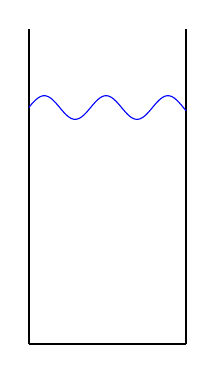
\begin{tikzpicture}[
      declare function={f1(\x) = 0.15 * sin(8.0 * deg(\x));
    }]

    \draw[thick] (0, 0) -- (0, 4);
    \draw[thick] (2, 0) -- (2, 4);
    \draw[thick] (0, 0) -- (2, 0);

    \begin{scope}[yshift=3cm, color=blue]
      \draw (0, 0) plot[domain=0:2, variable=\x, samples=200, smooth] ({\x}, {f1(\x)});
    \end{scope}

  \end{tikzpicture}
  \caption{Пример ёмкости с водой.}
  \label{fig:electronics-current-0}
\end{figure}

Вода в ёмкости имеет некоторую \emph{потенциальную энергию}, которая может быть
потрачена с какой-либо целью.  Например, если мы внизу ёмкости проделаем
отверстие, то вода из него будет вытекать
(см. рис. \ref{fig:electronics-current-1}); если при этом под струю воды
подставить водяное колесо, то таким образом можно приводить в движение
механизмы.

\begin{figure}[ht]
  \centering
  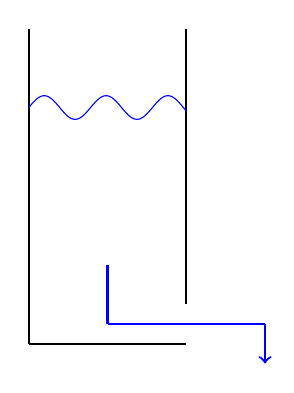
\begin{tikzpicture}[
      declare function={f1(\x) = 0.15 * sin(8.0 * deg(\x));
    }]

    \draw[thick] (0, 0) -- (0, 4);
    \draw[thick] (2, 0.5) -- (2, 4);
    \draw[thick] (0, 0) -- (2, 0);

    \draw[thick, color=blue] (1, 1) -- (1, 0.25);
    \draw[thick, color=blue] (1, 0.25) -- (3, 0.25);
    \draw[thick, color=blue, ->] (3, 0.25) -- (3, -0.25);

    \begin{scope}[yshift=3cm, color=blue]
      \draw (0, 0) plot[domain=0:2, variable=\x, samples=200, smooth] ({\x}, {f1(\x)});
    \end{scope}

  \end{tikzpicture}
  \caption{Пример ёмкости с водой и отверстием снизу.}
  \label{fig:electronics-current-1}
\end{figure}

Проводя аналогию с электричеством можно сказать, что ёмкость имеет некоторое
\emph{напряжение} воды.  В электрической батарее как правило запасена
\emph{химическая энергия}, которая может быть высвобождена при определённых
условиях.

Напряжение в электрической цепи измеряется в \emph{Вольтах} (В).

Таким образом, мы можем сделать первый вывод: для протекания тока необходим
некий источник тока, обладающий некоторым напряжением.

\end{document}
